\hypertarget{Reverb_8cpp}{
\section{Reverb.cpp File Reference}
\label{Reverb_8cpp}\index{Reverb.cpp@{Reverb.cpp}}
}
{\tt \#include $<$math.h$>$}\par
{\tt \#include \char`\"{}Sound\-Sample.h\char`\"{}}\par
{\tt \#include \char`\"{}Collection.h\char`\"{}}\par
{\tt \#include \char`\"{}Track.h\char`\"{}}\par
{\tt \#include \char`\"{}Multi\-Track.h\char`\"{}}\par
{\tt \#include \char`\"{}LPComb\-Filter.h\char`\"{}}\par
{\tt \#include \char`\"{}All\-Pass\-Filter.h\char`\"{}}\par
{\tt \#include \char`\"{}Reverb.h\char`\"{}}\par
{\tt \#include \char`\"{}Types.h\char`\"{}}\par


Include dependency graph for Reverb.cpp:\begin{figure}[H]
\begin{center}
\leavevmode
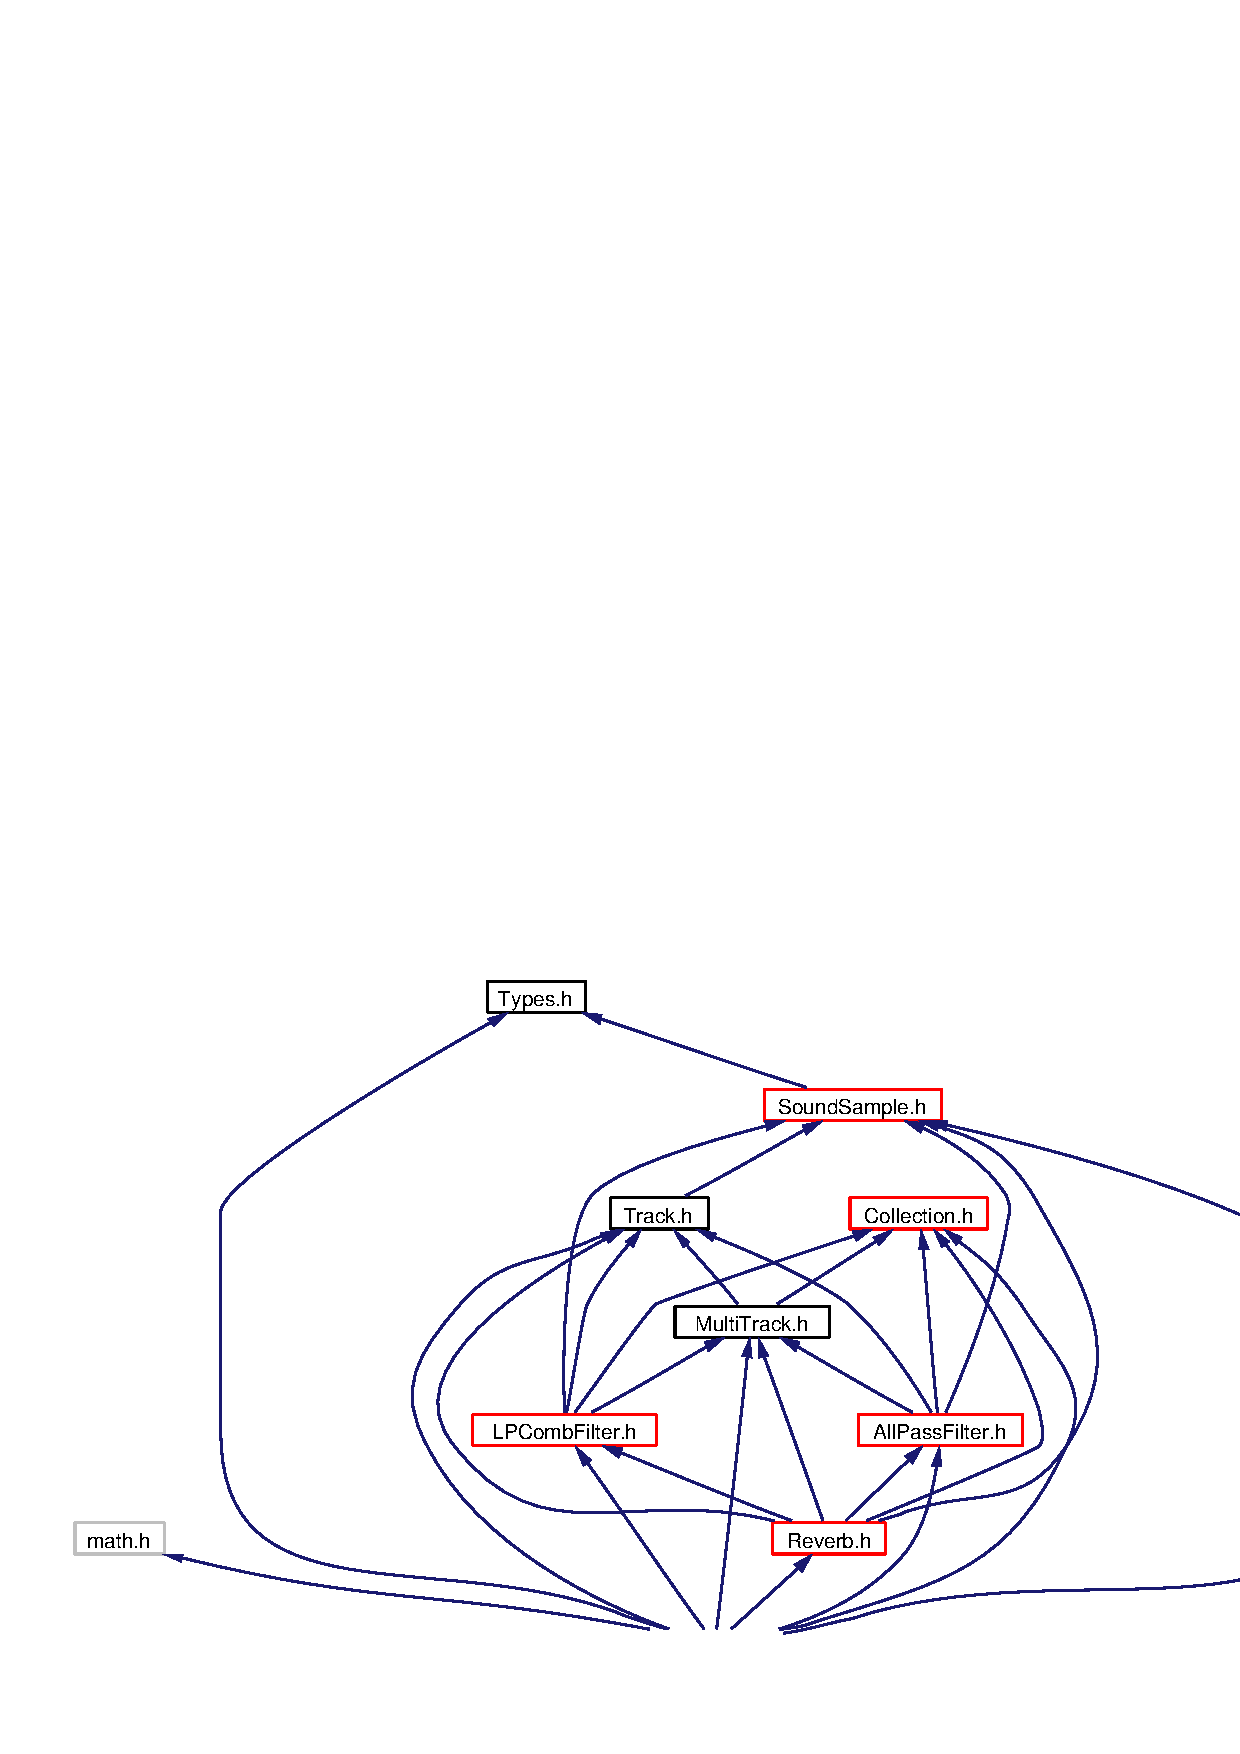
\includegraphics[width=332pt]{Reverb_8cpp__incl}
\end{center}
\end{figure}
\subsection*{Defines}
\begin{CompactItemize}
\item 
\#define \hyperlink{Reverb_8cpp_a0}{max}(x, y)\ ((x) $>$ (y) ? (x) : (y))
\end{CompactItemize}


\subsection{Define Documentation}
\hypertarget{Reverb_8cpp_a0}{
\index{Reverb.cpp@{Reverb.cpp}!max@{max}}
\index{max@{max}!Reverb.cpp@{Reverb.cpp}}
\subsubsection[max]{\setlength{\rightskip}{0pt plus 5cm}\#define max(x, y)\ ((x) $>$ (y) ? (x) : (y))}}
\label{Reverb_8cpp_a0}


